\documentclass[a4paper,12pt]{article}
\usepackage{HomeWorkTemplate}

\usepackage[utf8]{inputenc}
\usepackage[]{babel}

\setlength{\parindent}{4em}
\setlength{\parskip}{0.5em}

\renewcommand{\baselinestretch}{1.5}


\usepackage{caption}
\usepackage{subcaption}
\usepackage{graphicx}
\usepackage{float}
\usepackage[utf8]{inputenc}
\usepackage{lmodern, textcomp}
\usepackage{circuitikz}
\usepackage[shortlabels]{enumitem}
\usepackage{hyperref}
\usepackage{tikz}
\usepackage{amsmath}
\usepackage{amssymb}
\usepackage{tcolorbox}
\usepackage{graphicx}
\usepackage{xepersian}
\settextfont{XB Niloofar}
\usetikzlibrary{arrows,automata}
\usetikzlibrary{circuits.logic.US}
\usepackage{changepage}
\newcounter{problemcounter}
\newcounter{subproblemcounter}
\setcounter{problemcounter}{1}
\setcounter{subproblemcounter}{1}
\newcommand{\problem}[1]
{
	\subsection*{
		پرسش
		\arabic{problemcounter} 
		\stepcounter{problemcounter}
		\setcounter{subproblemcounter}{1}
		#1
	}
}
\newcommand{\subproblem}{
	\textbf{\harfi{subproblemcounter})}\stepcounter{subproblemcounter}
}


\begin{document}
\handout
{اصول پردازش تصویر}
{دکتر مصطفی کمالی تبریزی}
{نیم‌سال اول 1399\lr{-}1400}
{اطلاعیه}
{سیدعلیرضا خادم}
{97100398}
{تمرین سری چهارم - سوال اول}
زمان حدودی اجرا: 90 ثانیه
\section*{موارد لازم.}
برای اجرا لازم است تا تصویر 
\lr{texture1.jpg}
در مسیر
\lr{EX4\_Q1/}
قرار داشته باشد. همچنین در پیاده‌سازی این سوال از کتابخانه‌های 
\lr{cv2}
و
\lr{numpy}
استفاده شده است که قبل از اجرا بایستی این کتابخانه‌ها روی سیستم شما نصب باشد.
\section*{روند کلی حل.}
هدف سوال ساخت یک تصویر با اندازه 2500 پیکسل در 2500 پیکسل است که بافت آن مشابه بافتِ تصویر 
\lr{texture1.jpg}
در مسیر
\lr{EX4\_Q1/}
باشد. برای انجام این کار 2 ایده اولیه وجود داره : 1. 
\lr{resize}
کردن سمپل داده شده برای تولید عکس با سایز بزرگتر 2. 
\lr{build probability distribution}.
هر یک از این روش‌ها معایب خودشان رادارند و این معایب به اندازه‌ای در نتیجه نهایی تاثیرگذر  است که باعث می‌شود برای حل این سوال سراغ این روش‌ها نرویم. ما در این جا از روش 
\lr{Image Quilting}
برای حل سوال استفاده می‌کنیم. ایده ‌کلی این روش براساس این مشاهده است که "پیکسل‌های همسایه همبستگی زیادی با هم دارند". ‌بر اساس این مشاهده، در روش 
\lr{Image Quilting}
تصویر نهایی را به‌جای این که پیکسل به پیکسل بسازیم، بلوک به بلوک می‌سازیم. کلیات این ایده را در تصویر زیر می‌توانید مشاهده کنید.
\begin{figure}[H]
	\centering
	\begin{subfigure}{0.8\textwidth}
		\centering
		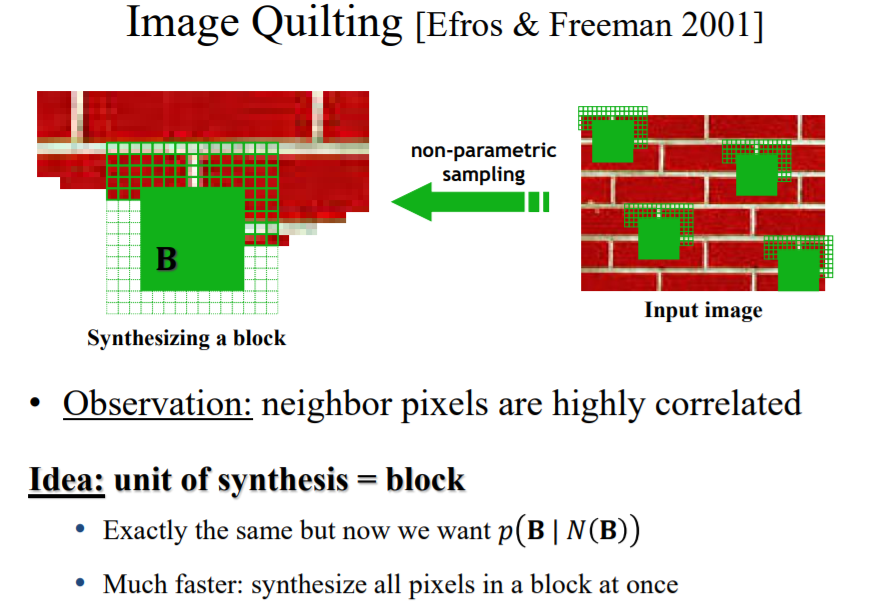
\includegraphics[width=.7\textwidth]{1.png}
	\end{subfigure}
\end{figure}
کاری که که انجام می‌دیم به این صورت است که در ابتدا یک 
\lr{block}
از تصویر 
\lr{sample}
را به صورت رندوم بر‌می‌داریم و در گوشه بالا سمت چپ تصویر 
\lr{target}
قرار می‌دهیم. (مشابه شکل زیر)
\begin{figure}[H]
	\centering
	\begin{subfigure}{0.8\textwidth}
		\centering
		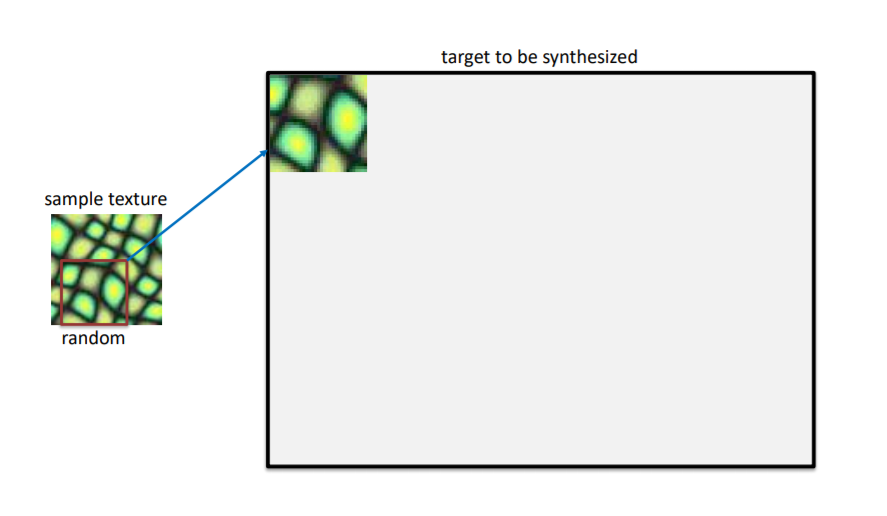
\includegraphics[width=.7\textwidth]{2.png}
	\end{subfigure}
\end{figure}
در ادامه یک 
\lr{patch}
جدید  از تصویر 
\lr{sample}
انتخاب می‌کنیم، اما نه کاملا به صورت رندوم، بلکه به این صورت که می‌خواهیم این 
\lr{patch}
جدید به گونه‌ای انتخاب بشود که سمت چپ آن تا حد زیادی مشابه سمت راستِ
\lr{patch}‌ای
که در مرحله قبل در تصویر 
\lr{target}
قرار داده‌ایم، باشد؛ بنابراین یک نوار از سمت راست 
 \lr{patch}ِ
 گام قبل در نظر می‌گیریم (مشابه عکس زیر) و همه 
 \lr{patch}‌های
 به ابعاد 
 \lr{patch}ِ
 گام قبل را که سمت چپشان شبیه به سمت راستِ 
 \lr{patch}
 گام قبل است را با یکی از روش‌های تمپلیت متچینگ (‌ما از روش 
 \lr{cv.TM\_CCORR\_NORMED}
 استفاده کردیم
 )پیدا می‌کنیم و از میان 
 \lr{patch}
 هایی که بیشترین شباهت را به 
 \lr{patch}ِ
 گام قبل دارند، یکی را به صورت رندوم انتخاب می‌کنیم.
 \begin{figure}[H]
 	\centering
 	\begin{subfigure}{0.5\textwidth}
 		\centering
 		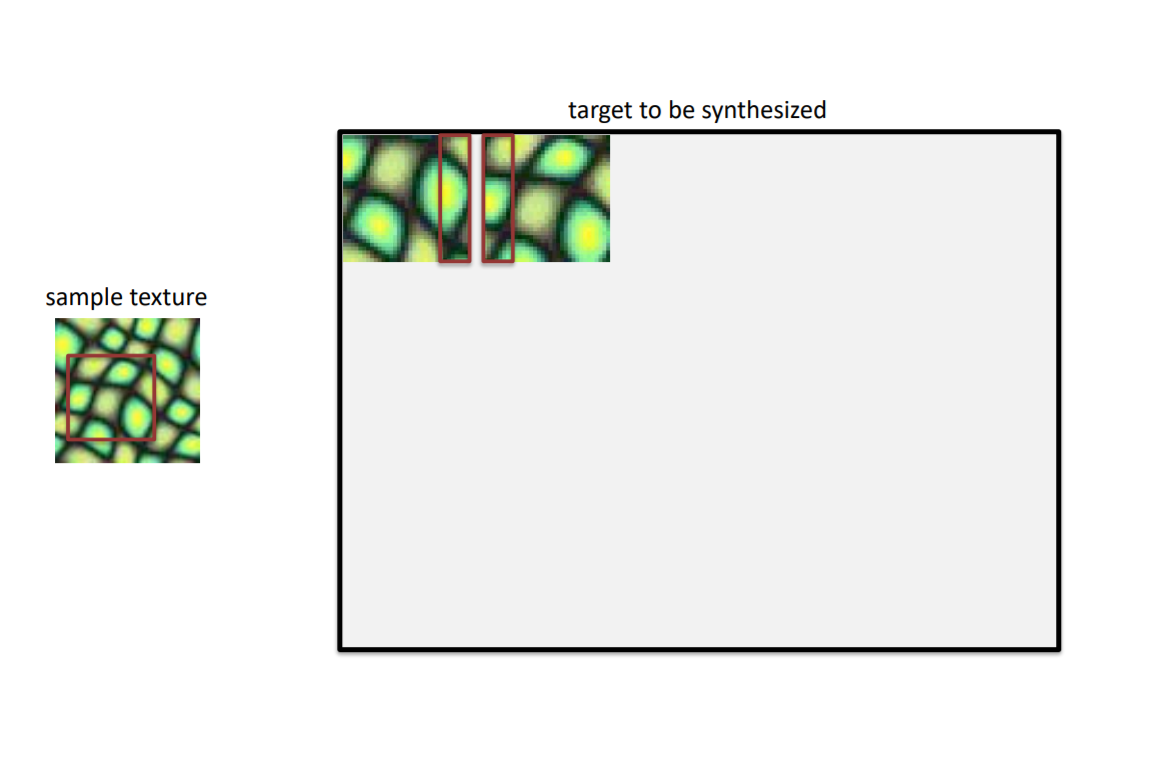
\includegraphics[width=.9\textwidth]{4.png}
 	\end{subfigure}%
	 \begin{subfigure}{0.5\textwidth}
	 	\centering
	 	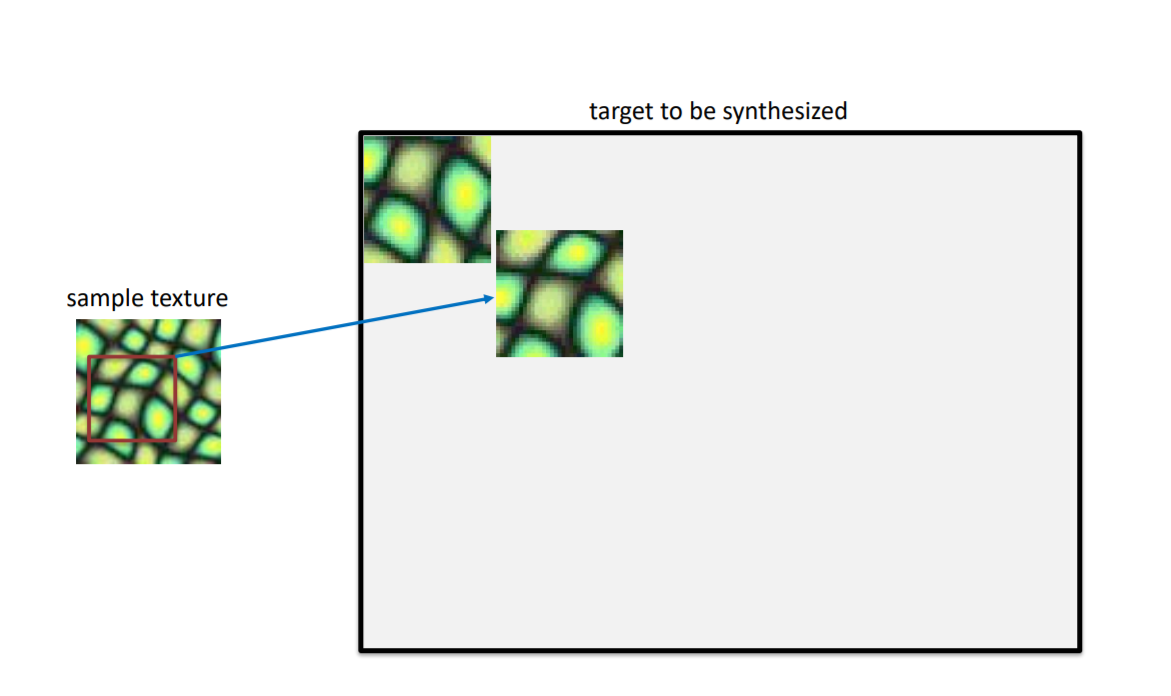
\includegraphics[width=.9\textwidth]{3.png}
	 \end{subfigure}%
 \end{figure}
بعد از اینکه 
\lr{patch}
جدید را انتخاب کردیم، در قسمتی که 
\lr{patch}
جدید و 
\lr{patch}
قبلی 
\lr{overlap}
دارند با استفاده از 
\lr{dynamic programing}
،
\lr{Minimum Cut}
را طبق تصاویر زیر اعمال می‌کنیم. سمت راستِ کات را از 
 \lr{patch}
 جدید و سمتِ چپ کات را از تصویر 
 \lr{target}
 بر‌می‌داریم.
\begin{figure}[H]
	\centering
	\begin{subfigure}{0.7\textwidth}
		\centering
		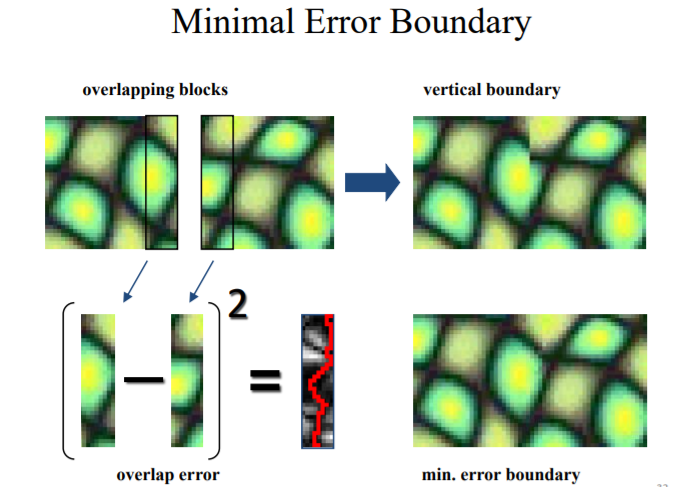
\includegraphics[width=.9\textwidth]{5.png}
	\end{subfigure}%
	\begin{subfigure}{0.3\textwidth}
		\centering
		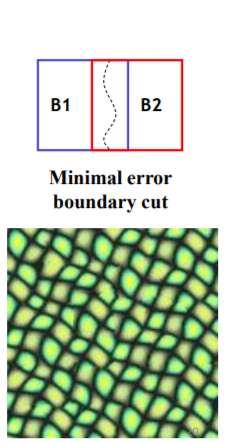
\includegraphics[width=.9\textwidth]{6.png}
	\end{subfigure}%
\end{figure}
روندی که در بالا توضیح داده شد را ادامه می‌دهیم تا سطر اول از تصویر
\lr{target}
ساخته شود. حال به سراغ سطر دوم می‌رویم. اولین 
\lr{patch}
از سطر دوم را که می‌خواهیم اضافه کنیم،‌ باید به این صورت عمل کنیم که یک نوار از بالایِ این
\lr{patch}
با یک نوار از پایینِ
\lr{patch}ِ
بالایی آن (مشابه عکس زیر) تا حدی خوبی مشابه باشند. و 
\lr{Min cut}
را توی این نوار اعمال می‌‌کنیم.
\begin{figure}[H]
	\centering
	\begin{subfigure}{0.33\textwidth}
		\centering
		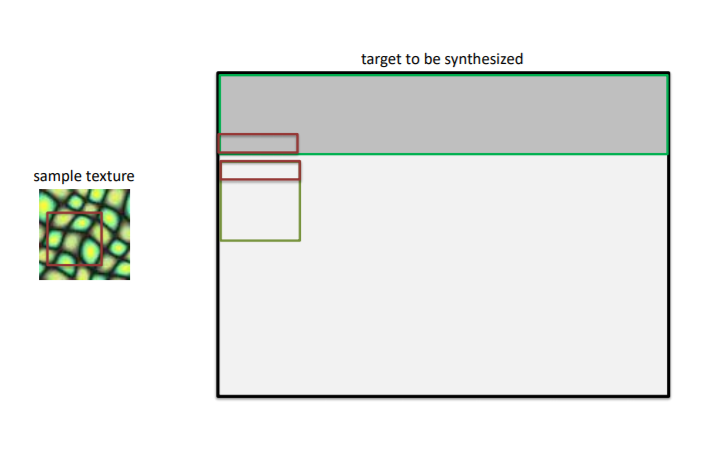
\includegraphics[width=\textwidth]{9.png}
	\end{subfigure}%
	\begin{subfigure}{0.33\textwidth}
		\centering
		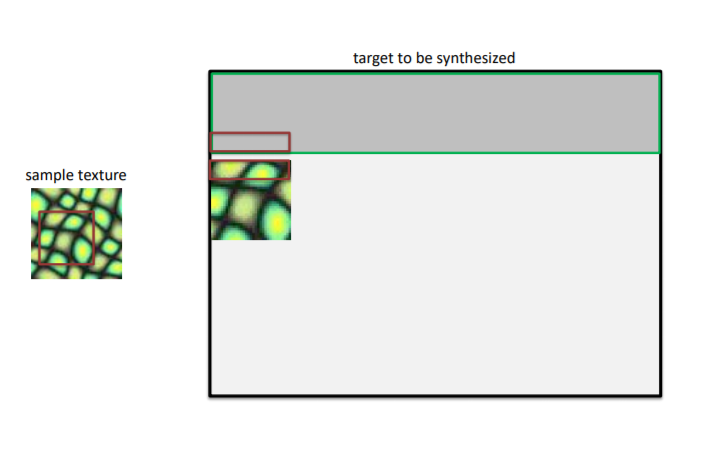
\includegraphics[width=\textwidth]{8.png}
	\end{subfigure}%
	\begin{subfigure}{0.33\textwidth}
		\centering
		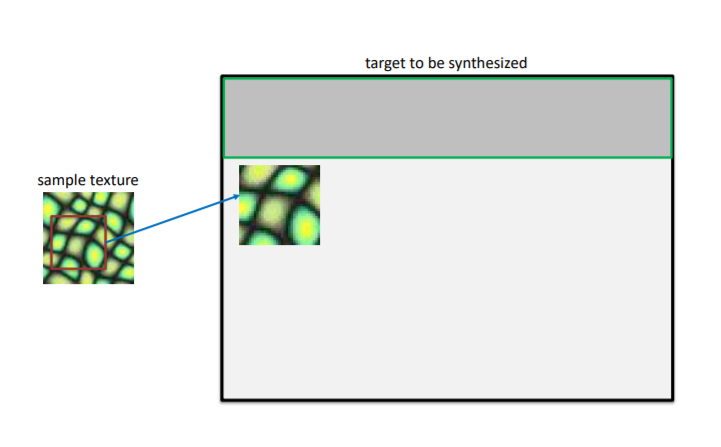
\includegraphics[width=\textwidth]{7.png}
	\end{subfigure}%
\end{figure}
در ادامه‌ی ساختِ سطر دوم، 
\lr{overlap}‌ای
که در نظر می‌گیریم تا بر اساس آن 
\lr{patch}
جدید را انتخاب کنیم به صورت
\lr{L}
شکل در نظر می‌گیریم(مشابه تصویر زیر). و در هر یک از نوار‌های بالا و سمت چپ 
\lr{Min cut}
را به دست می آوریم و جایی که این دو کات همگدیگر را قطع می‌کند را در نظر می‌گیریم و بالا‌یِ کاتِ افقی و سمت جپ کاتِ عمودی را از تصویر 
\lr{target}
و پایینِ کاتِ افقی و سمتِ راستِ کات عمودی را از 
\lr{patch}
جدید می آوریم.
 \begin{figure}[H]
	\centering
	\begin{subfigure}{0.2\textwidth}
		\centering
		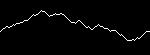
\includegraphics[width=0.6\textwidth]{13.png}
		\subcaption{کات افقی}
	\end{subfigure}%
	\begin{subfigure}{0.2\textwidth}
		\centering
		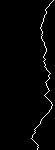
\includegraphics[width=0.3\textwidth]{12.png}
		\subcaption{کات عمودی}
	\end{subfigure}%
	\begin{subfigure}{0.2\textwidth}
		\centering
		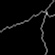
\includegraphics[width=0.4\textwidth]{11.png}
		\subcaption{تقاطع دو کات}
	\end{subfigure}%
\end{figure}
 \begin{figure}[H]
	\centering
	\begin{subfigure}{0.8\textwidth}
		\centering
		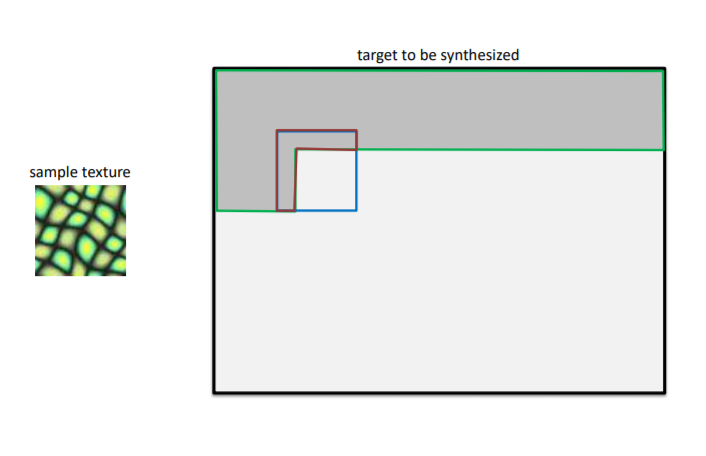
\includegraphics[width=.7\textwidth]{10.png}
	\end{subfigure}%
\end{figure}
روندی که در بالا برای سطر دوم توضیح دادیم را برای دیگر سطرها به صورت مشابه انجام می‌دهیم تا به طول کامل تصویر
\lr{target}
ساخته شود.


\section*{توضیح کد.}
برنامه در مجموع حاوی 2 فایل با فرمت
\lr{.py}
می‌باشد که توضیحات هر فایل در پایین آمده است.
\subsection*{$\circ$ utilities.py}

\subsubsection*{\lr{initialized\_first\_block(src\_image, target\_image, height\_of\_block, width\_of\_block)}}
در این تابع ورودی‌های
\lr{src\_image}
،
\lr{target\_image}
،
\lr{height\_of\_block}
و
\lr{width\_of\_block}
را می‌گیرد و یک 
\lr{patch}
به ابعاد \lr{height\_of\_block } $ \times $\lr{width\_of\_block } به صورت تصادفی از تصویر 
\lr{src\_image}
برمی‌دارد و در گوشه‌یِ بالا سمت چپ تصویر
\lr{target}
قرار می‌دهد.

\begin{figure}[H]
\centering
\begin{subfigure}{0.8\textwidth}
	\centering
	
\includegraphics[width=.4\textwidth]{18.jpg}
	\subcaption{mask}
\end{subfigure}%
\end{figure}
\subsubsection*{\lr{find\_matching(src\_image, patch, height\_of\_block, width\_of\_block)}}
 این تابع ورودی‌هایی که مشخص شده است را می‌گیرد و تصویر
 \lr{patch}
 را داخل تصویر
 \lr{src\_image}
 با روش \\
 \lr{cv.TM\_CCORR\_NORMED}
 سرچ می‌زند و نتیجه را در متغیر 
 \lr{matching}
 ذخیره می‌کند. در ادامه آن پیکسل‌هایی از 
  \lr{matching}
  که مقدار آن از 
  \lr{matching.max() - .0001}
  بیشتر بود را به عنوان کاندیدِ آن قسمت‌هایی از 
  \lr{src\_image}
  که بیشترین شباهت را به 
  ‌\lr{patch}
  را دارد در متغیر 
  \lr{locations}
  ذخیره می‌کند. در نهایت هم یک قسمت از تصویر 
  \lr{src\_image}
  را به عنوان یکی از قسمت که بیشترین شباهت را به 
  \lr{patch}
  دارد به صورت تصادفی از میان مختصات‌هایِ 
  \lr{locations}
   انتخاب کرده و به عنوان خروجی بر‌می‌گرداند.
   \subsubsection*{\lr{find\_l\_matching(src\_image, patch, height\_of\_block, width\_of\_block, overlap)}}
   این تابع مشابه تابع 
    \lr{find\_matching}
    است با این تفاوت که کاربرد آن در مواقعی است که اورلپ به صورت L شکل است. این تابع ورودی‌هایی که مشخص شده است را می‌گیرد و تصویر
   \lr{patch}
   را داخل تصویر
   \lr{src\_image}
   با روش \\
   \lr{cv.TM\_CCORR\_NORMED}
    و با در نظر گرفتنِ 
    \lr{mask}‌ای
    که در ادامه تصویر آن آمده است سرچ می‌زند و نتیجه را در متغیر 
   \lr{matching}
   ذخیره می‌کند. در ادامه آن پیکسل‌هایی از 
   \lr{matching}
   که مقدار آن از 
   \lr{matching.max() - .0001}
   بیشتر بود را به عنوان کاندیدِ آن قسمت‌هایی از 
   \lr{src\_image}
   که بیشترین شباهت را به 
   ‌\lr{patch}
   را دارد در متغیر 
   \lr{locations}
   ذخیره می‌کند. در نهایت هم یک قسمت از تصویر 
   \lr{src\_image}
   را به عنوان یکی از قسمت که بیشترین شباهت را به 
   \lr{patch}
   دارد به صورت تصادفی از میان مختصات‌هایِ 
   \lr{locations}
   انتخاب کرده و به عنوان خروجی بر‌می‌گرداند.
   \subsubsection*{\lr{vertically\_min\_cut(first\_patch, second\_patch)}}
   این تابع برای محاسبه‌یِ کاتِ عمودی در ساختن سطر اول از 
   \lr{target}
   استفاده می‌شود؛‌ مواردی که اورلپ تنها شامل یک نوار عمودی می‌شود (این شرایط در سطر اول اتفاق می‌افتد).در این تابع 
   \lr{first\_patch}
   و
   \lr{second\_patch}
   را به عنوان ورودی می‌گیرد و مین کات را محاسبه می‌کند به این صورت که مجذورِ تفاضل دو 
   \lr{patch}
   را در متغیر 
   \lr{difference\_of\_squares}
   ذخیره می‌کند و در ادامه با استفاده از 
    \lr{dynamic programing}
    یک مین کات عمودی را محاسبه می‌کند و در نهایت تصویری را به عنوان خروجی بر‌می‌گرداند که خود کات و سمت راست کات را از 
     \lr{second\_patch}
     و سمت چپ کات را از 
     \lr{first\_patch}
     قرار داده است.
      \subsubsection*{\lr{horizontally\_min\_cut(first\_patch, second\_patch)}}
     این تابع برای محاسبه‌یِ کاتِ افقی در ساختن ستون اول از 
     \lr{target}
     استفاده می‌شود؛‌ مواردی که اورلپ تنها شامل یک نوار افقی می‌شود (این شرایط در سطر اول اتفاق می‌افتد).در این تابع 
     \lr{first\_patch}
     و
     \lr{second\_patch}
     را به عنوان ورودی می‌گیرد و مین کات را محاسبه می‌کند به این صورت که مجذورِ تفاضل دو 
     \lr{patch}
     را در متغیر 
     \lr{difference\_of\_squares}
     ذخیره می‌کند و در ادامه با استفاده از 
     \lr{dynamic programing}
     یک مین کات افقی را محاسبه می‌کند و در نهایت تصویری را به عنوان خروجی بر‌می‌گرداند که خود کات و بالای کات را از 
     \lr{first\_patch}
     و پایین کات را از 
     \lr{second\_patch}
     قرار داده است.
     \subsubsection*{\lr{vertically\_min\_cut2(first\_patch, second\_patch)}}
     این تابع برای محاسبه‌یِ کاتِ عمودی در ساختن سطر‌های دوم به بعد و ستون‌های دوم به بعد از 
     \lr{target}
     مورد استفاده قرار می‌گیرد. مواردی که اورلپ به صورت L شکل است.در این تابع 
     \lr{first\_patch}
     و
     \lr{second\_patch}
     را به عنوان ورودی می‌گیرد و مین کات را محاسبه می‌کند به این صورت که مجذورِ تفاضل دو 
     \lr{patch}
     را در متغیر 
     \lr{difference\_of\_squares}
     ذخیره می‌کند و در ادامه با استفاده از 
     \lr{dynamic programing}
     یک مین کات عمودی را محاسبه می‌کند و در نهایت تصویری را به عنوان خروجی بر‌می‌گرداند که خود کات و سمت راست کات درآیه‌های صفر
     و سمت چپ کات را از 
     \lr{first\_patch}
     قرار داده است. علاوه بر آن کات رو هم مشابه شکل زیر به عنوان خروجی برمی‌گرداند.
      \begin{figure}[H]
     	\centering
     	\begin{subfigure}{0.2\textwidth}
     		\centering
     		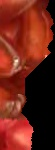
\includegraphics[width=0.4\textwidth]{15.jpg}
     		\subcaption{کات خروجی}
     	\end{subfigure}%
     	\begin{subfigure}{0.2\textwidth}
     		\centering
     		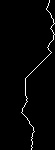
\includegraphics[width=0.4\textwidth]{14.jpg}
     		\subcaption{تصویر خروجی}
     	\end{subfigure}%
     \end{figure}
     \subsubsection*{\lr{horizontally\_min\_cut2(first\_patch, second\_patch)}}
          این تابع برای محاسبه‌یِ کاتِ افقی در ساختن سطر‌های دوم به بعد و ستون‌های دوم به بعد از 
     \lr{target}
     مورد استفاده قرار می‌گیرد. مواردی که اورلپ به صورت L شکل است.در این تابع 
     \lr{first\_patch}
     و
     \lr{second\_patch}
     را به عنوان ورودی می‌گیرد و مین کات را محاسبه می‌کند به این صورت که مجذورِ تفاضل دو 
     \lr{patch}
     را در متغیر 
     \lr{difference\_of\_squares}
     ذخیره می‌کند و در ادامه با استفاده از 
     \lr{dynamic programing}
     یک مین کات افقی را محاسبه می‌کند و در نهایت تصویری را به عنوان خروجی بر‌می‌گرداند که خود کات و  پایین آن درآیه‌های صفر
     و بالایِ کات را از 
     \lr{first\_patch}
     قرار داده است. علاوه بر آن کات رو هم مشابه شکل زیر به عنوان خروجی برمی‌گرداند.
     \begin{figure}[H]
     	\centering
     	\begin{subfigure}{0.2\textwidth}
     		\centering
     		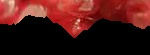
\includegraphics[width=0.95\textwidth]{17.jpg}
     		\subcaption{کات خروجی}
     	\end{subfigure}%
     	\begin{subfigure}{0.2\textwidth}
     		\centering
     		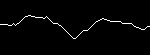
\includegraphics[width=0.95\textwidth]{16.jpg}
     		\subcaption{تصویر خروجی}
     	\end{subfigure}%
     \end{figure}
 \subsubsection*{\lr{texture\_synthesis(src\_image, target\_image, height\_of\_block, width\_of\_block, overlap)}}
 در این تابع با استفاده از توابعی که تا به اینجا توضیح داده شد و بر اساس روندی که در قسمت 
 \textbf{روند کلی حل.}
 بررسی شد 
\lr{texture}ِ
را تولید می‌کند.
 
\subsection*{$\circ$ q1.py}
در این فایل ابتدا تصویر 
 \lr{texture1.jpg}
را از مسیر
 \lr{EX4\_Q1/images/}
لود می‌کنیم و در متغیر 
\lr{src\_image}
قرار می‌دهیم و بعد آرایه 3 بعدی $ 2700 \times 2700 \times 3 $
\lr{target}
که همه درآیه‌های آن صفر است را تعریف می‌کنیم. در نهایت با فراخوانی تابع 
\lr{texture\_synthesis}
روی ورودی‌هایی که مشاهده می‌کنید، 
\lr{target}
را با 
\lr{patch}‌های
$ 150 \times 150 $
که $ 55 $ پیکسل پهنایِ نوارهای 
\lr{overlap}
آنهاست‌، پرمی‌کنیم. در آخر هم نتیجه را با نام 
\lr{res01.jpg}
در مسیر
\lr{EX4\_Q1/results/}
ذخیره می‌کنیم.	

\end{document}
